\chapter{Introdução}
\label{ch:introducao}

\textit{\textcolor{red}{Sugere-se apresentar um texto adequadamente conciso, com a contextualização e justificativa do tema do trabalho. Importante que o candidato traga de forma geral, e contextualizada, a importância do tema da pesquisa, citar trabalhos relevantes já desenvolvidos. Adicionalmente, apresentar no último parágrafo da Introdução, antes do item objetivo, de forma conectada, a justificativa do estudo, ressaltando os impactos do mesmo.}}

\textit{\textcolor{red}{O texto deve evitar o aprofundamento ou detalhamento. A introdução deve contextualizar, apresentar os problemas, deficiências ou oportunidades de melhoria e justificar os objetivos a serem apresentados na sequencia.}}

Os textos em \textit{\textcolor{red}{vermelho e itálico}} são mais sobre a parte de orientação para preenchimento de cada tópico ~\cite{abadi2016tensorflow}.

\begin{figure}
    \caption{Exemplo de imagem.}
    \centering
    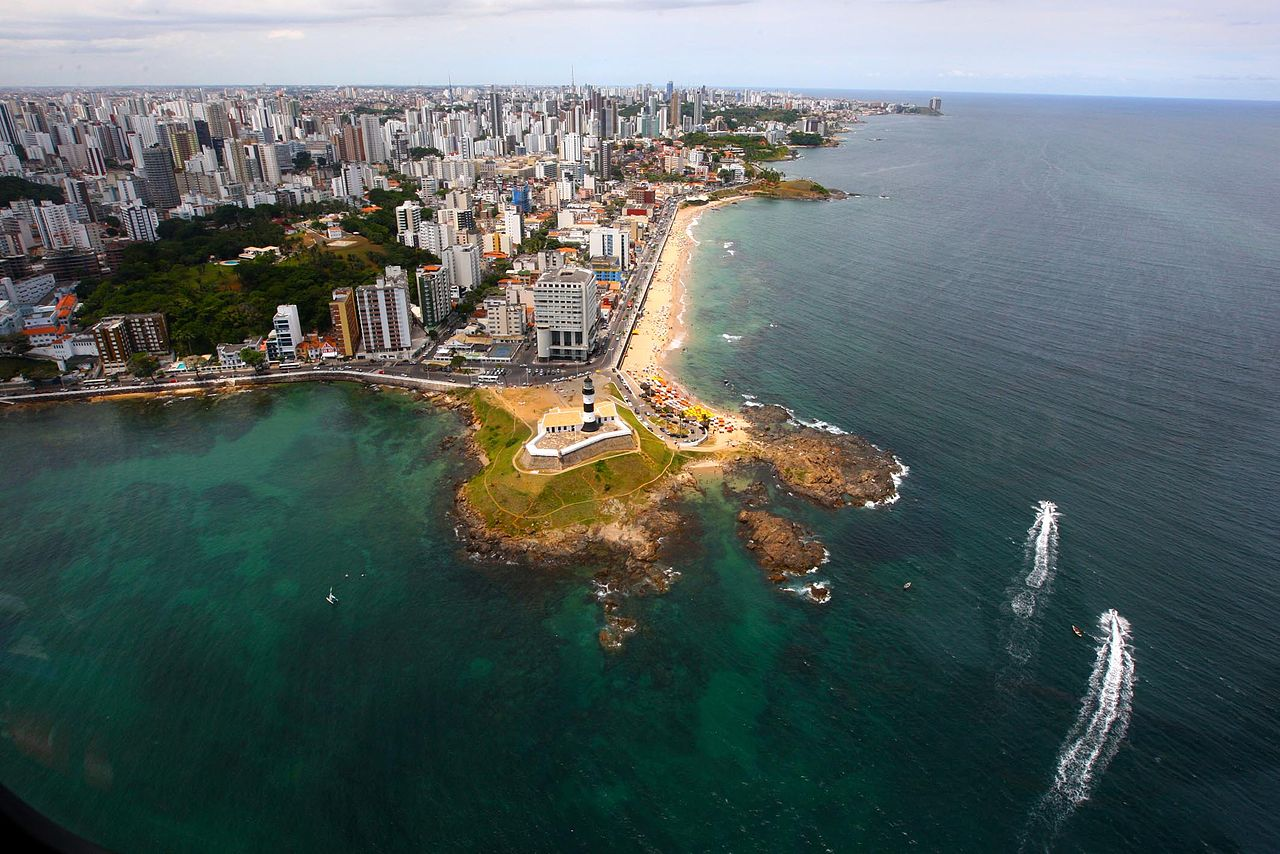
\includegraphics[width=0.6\textwidth]{images/farol_da_barra.jpg}
    \fbe{pedregosa2011scikit}
    \label{fig:seismic_acq}
\end{figure}

\lipsum[1-1]

\begin{figure}
    \caption{Exemplo de imagem.}
    \centering
    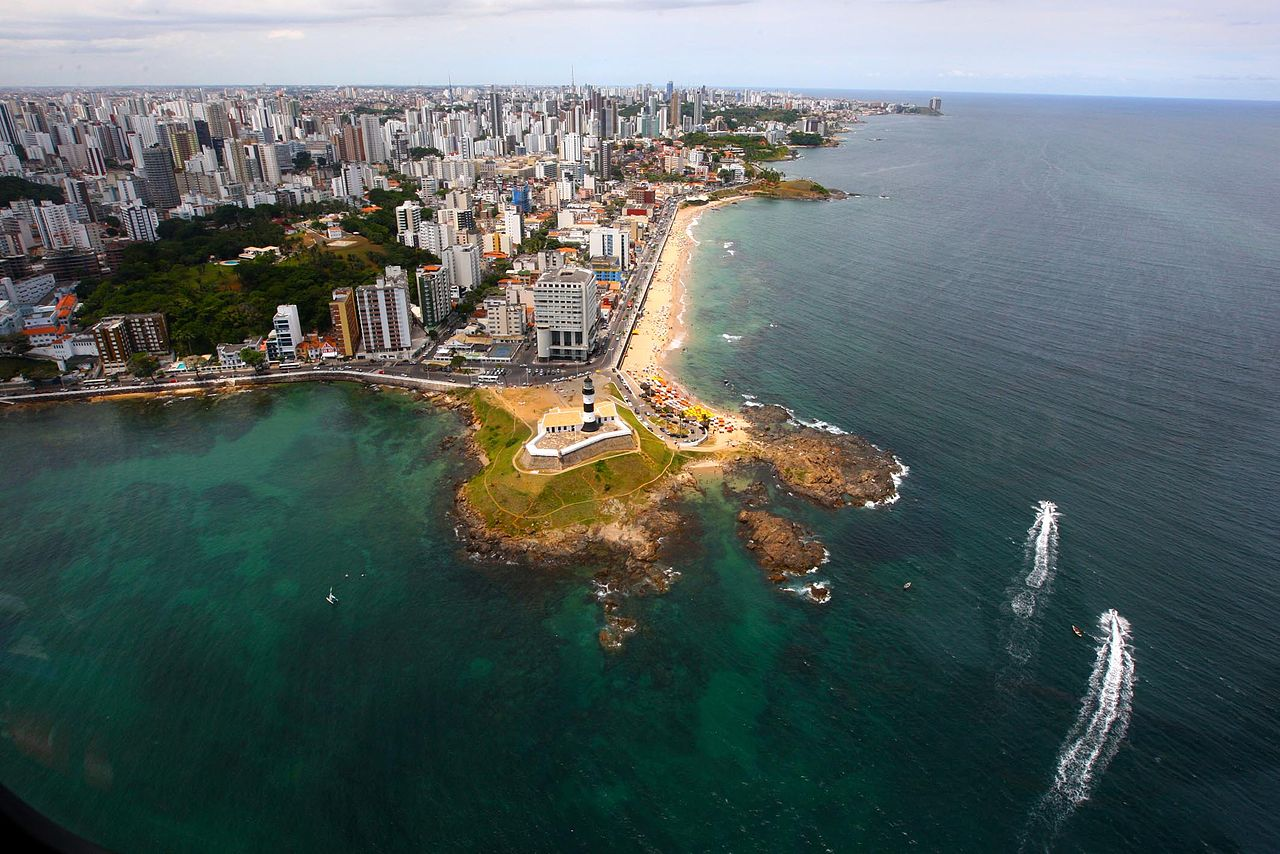
\includegraphics[width=0.6\textwidth]{images/farol_da_barra.jpg}
    \fea
    \label{fig:fig_exemplo_2}
\end{figure}

\lipsum[2-2]

\begin{enumerate}
    \item Item 1... ;
    \item Item 2... .
\end{enumerate}

\lipsum[3-3]

\section{Objetivo}
\label{section:objetivo}

\textit{\textcolor{red}{Apresentar o objetivo geral da Tese ou dissertação. Este precisa estar bem conectado com título do trabalho.}} O objetivo deste trabalho é...

\section{Objetivos Específicos}
\textit{\textcolor{red}{Apresentar os objetivos específicos da tese ou dissertação (em tópicos) – Lembre-se que TODOS os objetivos específicos devem ser respondidos na conclusão. Use uma sequência adequada que represente a apresentação de seus resultados.}}
Para alcançar o objetivo do trabalho, foi proposto como objetivos específicos:
\begin{enumerate}
    \item Realizar...;
    \item Desenvolver...;
    \item Analisar...;
    \item ... .
\end{enumerate}

\section{Organização do Documento}
\label{section:organizacao}
\textit{\textcolor{red}{Sugere-se que seja feita uma breve descrição do que o leitor irá encontrar em cada capítulo do trabalho.}}

Este trabalho está disposto de acordo com os seguintes capítulos:

\begin{itemize}
    \item \textbf{Capítulo \ref{ch:introducao} - \nameref{ch:introducao}}: \textit{\textcolor{red}{bla bla}}
  
    \item \textbf{Capítulo \ref{ch:revisao_literatura} - \nameref{ch:revisao_literatura}}: \textit{\textcolor{red}{bla bla}}
  
    \item \textbf{Capítulo \ref{chapther:metodologia} - \nameref{chapther:metodologia}}: \textit{\textcolor{red}{bla bla}}
    
    \item \textbf{Capítulo \ref{ch:resultados_discussao} - \nameref{ch:resultados_discussao}}: \textit{\textcolor{red}{bla bla}}
    
    \item \textbf{Capítulo \ref{ch:conclusoes} - \nameref{ch:conclusoes}}: \textit{\textcolor{red}{bla bla}}
\end{itemize}